\documentclass[12pt,                    % corpo del font principale
               a4paper,                 % carta A4
               twoside,                 % impagina per fronte-retro
               openright,               % inizio capitoli a destra
               english,                 
%                italian,                 
               ]{book}    


% codifica di input; anche [latin1] va bene
% NOTA BENE! va accordata con le preferenze dell'editor
\usepackage[utf8]{inputenc}

%**************************************************************
% Importazione package
%************************************************************** 

%\usepackage{amsmath,amssymb,amsthm}    % matematica


% per scrivere in italiano e in inglese;
% l'ultima lingua (l'italiano) risulta predefinita
% \usepackage[english, italian]{babel}    
\usepackage[english]{babel}

\usepackage{bookmark}                   % segnalibri

\usepackage{caption}                    % didascalie

\usepackage{chngpage,calc}              % centra il frontespizio

% gestisce automaticamente i caratteri (")
\usepackage{csquotes}                  

% pagine vuote senza testatina e piede di pagina
\usepackage{emptypage}                  

\usepackage{epigraph}					% per epigrafi

\usepackage{eurosym}                    % simbolo dell'euro

% codifica dei font:
% NOTA BENE! richiede una distribuzione *completa* di LaTeX
\usepackage[T1]{fontenc}                

% rientra il primo paragrafo di ogni sezione
%\usepackage{indentfirst}              

\usepackage{graphicx}                   % immagini

\usepackage{breakurl}
%\usepackage{hyperref}                   % collegamenti ipertestuali


% margini ottimizzati per l'A4; rilegatura di 5 mm
\usepackage[binding=5mm]{layaureo}      

\usepackage{listings}                   % codici
\usepackage{courier}

\usepackage{microtype}                  % microtipografia

\usepackage{mparhack,relsize}  % finezze tipografiche

\usepackage{nameref}                    % visualizza nome dei riferimenti

\usepackage[font=small]{quoting}        % citazioni

%\usepackage{subfig}                     % sottofigure, sottotabelle

% \usepackage[italian]{varioref}          % riferimenti completi della pagina
\usepackage[english]{varioref}

%\usepackage[dvipsnames]{color}         % colori

\usepackage{booktabs}                   % tabelle
\usepackage{tabularx}                   % tabelle di larghezza prefissata
\usepackage{longtable}                  % tabelle su più pagine
% tabelle su più pagine e adattabili in larghezza
\usepackage{ltxtable}                   

% glossario
% per includerlo nel documento bisogna:
% 1. compilare una prima volta tesi.tex;
% 2. eseguire: makeindex -s tesi.ist -t tesi.glg -o tesi.gls tesi.glo
% 3. eseguire: makeindex -s tesi.ist -t tesi.alg -o tesi.acr tesi.acn
% 4. compilare due volte tesi.tex.
\usepackage[toc, acronym]{glossaries}

% eccellente pacchetto per la bibliografia; 
% produce uno stile di citazione autore-anno; 
% lo stile "numeric-comp" produce riferimenti numerici
% per includerlo nel documento bisogna:
% 1. compilare una prima volta tesi.tex;
% 2. eseguire: biber tesi
% 3. compilare ancora tesi.tex.
\usepackage[backend=biber,sorting=none,style=numeric,hyperref,backref]{biblatex}

% permette di inserire le immagini/tabelle esattamente dove viene usato il
% comando \begin{figure}[H] ... \end{figure}
% evitando che venga spostato in automatico
\usepackage{float}

\usepackage{bold-extra}

\usepackage{etoolbox}

\usepackage{catchfile}
\newcommand{\getenv}[2][]{%
  \CatchFileEdef{\temp}{"|kpsewhich --var-value #2"}{}%
  \if\relax\detokenize{#1}\relax\temp\else\let#1\temp\fi}

\usepackage{ifthen}
\usepackage{todonotes}

% aggiunto per avere enumeration e itemize inline
\usepackage[inline]{enumitem}

% titoli dei capitoli personalizzati
\usepackage[explicit]{titlesec}

% part personalizzata
\usepackage{lmodern}
\usepackage{tikz}
\usepackage{wrapfig}

% Multi-column
\usepackage{etoolbox,refcount}

% scrittura su più di una colonna
\usepackage{multicol}

% Marging notes
\usepackage{marginnote}
\usepackage{subcaption}

% to add a pdf
\usepackage{pdfpages}
%**************************************************************
% file contenente le impostazioni della tesi
%**************************************************************

%**************************************************************
% Frontespizio
%**************************************************************
\newcommand{\myName}{Name Surname}                                    % autore
\newcommand{\myTitle}{A thesis}                                 % tipo di tesi
\newcommand{\mySupervisor}{Name Surname}                        % relatore
\newcommand{\myCoSupervisor}{Name Surname}                      % co-relatore
% decomment line 12 or 13
\newbool{ifCoSupervisor}
\booltrue{ifCoSupervisor}
% \boolfalse{ifCoSupervisor}
\newcommand{\myDegree}{Tesi di laurea magistrale}                
\newcommand{\myUni}{Università degli Studi di Padova}           % università
\newcommand{\myFaculty}{Corso di Laurea in Informatica}         % facoltà
\newcommand{\myDepartment}{Dipartimento di Matematica}          % dipartimento
\newcommand{\myLocation}{Padova}                                % dove
\newcommand{\myAA}{2017-2018}                                   % anno
\newcommand{\myTime}{December 2018}                             % quando


%**************************************************************
% Impostazioni di impaginazione
% see: http://wwwcdf.pd.infn.it/AppuntiLinux/a2547.htm
%**************************************************************

\setlength{\parindent}{14pt}   % larghezza rientro della prima riga
\setlength{\parskip}{0pt}   % distanza tra i paragrafi


%**************************************************************
% Impostazioni di biblatex
%**************************************************************
\bibliography{res/bibliography} % database di biblatex

\defbibheading{bibliography}
{
    \cleardoublepage
    \phantomsection
    \addcontentsline{toc}{chapter}{\bibname}
    \chapter*{\bibname\markboth{\bibname}{\bibname}}
}

\setlength\bibitemsep{1.5\itemsep} % spazio tra entry

% \DeclareBibliographyCategory{opere}
% \DeclareBibliographyCategory{web}
% 
% \addtocategory{web}{site:agile-manifesto}
% \addtocategory{web}{site:aws-lambda}
% \addtocategory{web}{site:aws-api-gateway}
% \addtocategory{web}{site:apex}
% \addtocategory{web}{site:swagger}
% \addtocategory{web}{site:messenger-facebook}
% \addtocategory{web}{site:aws-dynamodb}
% \addtocategory{web}{site:mocha}
% 
% \defbibheading{web}{\section*{Siti Web consultati}}


%**************************************************************
% Impostazioni di caption
%**************************************************************
\captionsetup{
    tableposition=top,
    figureposition=bottom,
    font=small,
    format=hang,
    labelfont=bf
}

%**************************************************************
% Impostazioni di glossaries
%**************************************************************
\newglossaryentry{nosql} {
  name=NoSQL,
  description={
NoSQL (Not Only SQL) è il nome di un tipo di DBMS che non prevede soltanto
l'utilizzo del modello relazionale utilizzato dai sistemi classici di tipo SQL.
}
}

\newglossaryentry{javascript_object_notation} {
  name=JavaScript Object Notation,
  description={
Formato adatto all’interscambio di dati fra applicazioni client-server. La
semplicità di JSON ne ha decretato un rapido utilizzo specialmente nella
programmazione in AJAX (Asynchronous JavaScript and XML). Il suo uso tramite
JavaScript è particolarmente semplice e questo fatto lo ha reso velocemente
molto popolare.
}
}

\newglossaryentry{url} {
  name=URL,
  description={
URL (Uniform Resource Locator) indica, specificando la posizione di una macchina
collegata alla rete internet e il meccanismo per ottenerla, un indirizzo a una
risorsa web.
}
}

\newglossaryentry{crud} {
  name=CRUD,
  description={
CRUD (Create, Read, Update and Delete) indica le operazioni effettuabili su
dispositivi di memoriazzazione. Nel contesto web, questo termine è stato
associato alle operazioni del protocollo HTTP.
}
}

\newglossaryentry{cloud} {
  name=Cloud,
  description={
Il cloud computing è un tipo di computing basato su internet, che provvede a
fornire risorse e informazioni ad altri computer su richiesta. È un modello di
computing che permette di configurare risorse in maniera rapida, basandosi
sulla condivisione di potenza di calcolo e virtualizzazione. Questo tipo di
modello permette ad aziende di creare la propria infrastruttura in maniera
flessibile, senza avere degli alti costi iniziali e gestionali.
}
}

\newglossaryentry{serverless} {
  name=Architettura serverless,
  description={
Un'architettura serverless è un tipo di cloud computing dove il gestore del
servizio cloud gestisce l'avvio e lo spegnimento delle macchine virtuali
necessarie per gestire le richieste, le risorse necessarie per il loro
funzionamento e la manutenzione dei sistemi. Questo, a differenza del nome, non
indica il fatto che non siano presenti server, ma indica il fatto che colui che
usufruisce di questo tipo di servizio non deve comprare o affittare alcun tipo
di macchine (reali o virtuali) per eseguire il proprio codice.
}
}

\newglossaryentry{api} {
  name=API,
  description={
Acronimo di \textit{Application Programming Interface}, indica un insieme
di procedure, funzionalità e protocolli per costruire programmi e applicazioni.
}
}

\newglossaryentry{yaml} {
  name=YAML,
  description={
Acronimo di \textit{YAML Ain't Markup Language}, ed è un formato file
per la serializzazione di dati utilizzabile dagli esseri umani. Nato nel 2001,
è stato progettato per l'inserimento di dati sottoforma di liste e array
associativi. È soprattutto impiegato nei file di configurazione e
presenta una buona facilità di lettura.
}
}

\newglossaryentry{agile} {
  name=Agile,
  description={
Insieme di principi per lo sviluppo software sotto i quali requisiti e
soluzioni evolvono tramite gli sforzi collettivi del gruppo auto-organizzato
polifunzionale.
}
}

\newglossaryentry{scrum} {
  name=Scrum,
  description={
SDLC iterativo-incrementale concepito per rilasci brevi e programmati del
software. L'obiettivo di Scrum è essere flessibile al cambio dei requisiti
imposti dal cliente, in modo da poter soddisfare al meglio le richieste
mantenendo un controllo sulla qualità e le tempistiche del progetto.
}
}

%Definizione presa da:
%https://it.wikipedia.org/wiki/Scrum_(informatica)
\newglossaryentry{scrumMaster} {
  name=Scrum Master,
  description={
Colui che facilita una corretta esecuzione dei processi di sviluppo. Lo Scrum
Master detiene l'autorità relativa all'applicazione delle norme, spesso
presiede le riunioni importanti e pone sfide alla squadra per migliorarla.
}
}

\newglossaryentry{startup}
{
  name=Startup,
  text=startup,
  sort=startup,
  description={
In economia, con questo termine, si indica una nuova impresa
nelle forme di un'organizzazione temporanea o una società di capitali in cerca
di un business model ripetibile e scalabile.
La scalabilità è un elemento cardine di questa tipologia di impresa. L'avvio di
un'attività imprenditoriale non scalabile, come l'apertura di un ristorante,
non coincide dunque con la creazione di una startup ma, piuttosto, di una
società tradizionale
}
}


% Acronimi
\newacronym{ceo}{CEO}{Chief Executive Officer}
\newacronym{cto}{CTO}{Chief Technology Officer}
\newacronym{ram}{RAM}{Random Access Memory}
\newacronym{rest}{REST}{Representational State Transfer}
\newacronym{soap}{SOAP}{Simple Object Access Protocol}
\newacronym{xml}{XML}{Extensible Markup Language}
\newacronym{http}{HTTP}{Hypertext Transfer Protocol}
\newacronym{mime}{MIME}{Multipurpose Internet Mail Extensions}
\newacronym{arn}{ARN}{Amazon Resource Name}
\newacronym{npm}{NPM}{Node Package Manager}
 % database di termini
\makeglossaries


%**************************************************************
% Impostazioni di graphicx
%**************************************************************
\graphicspath{{res/img/}} % cartella dove sono riposte le immagini


%**************************************************************
% Impostazioni di hyperref
%**************************************************************
\hypersetup{
    %hyperfootnotes=false,
    %pdfpagelabels,
    %draft,	% = elimina tutti i link (utile per stampe in bianco e nero)
    colorlinks=true,
    linktocpage=true,
    pdfstartpage=1,
    pdfstartview=FitV,
    % decommenta la riga seguente per avere link in nero (per esempio per la
%stampa in bianco e nero)
    %colorlinks=false, linktocpage=false, pdfborder={0 0 0}, pdfstartpage=1,
%pdfstartview=FitV,
    breaklinks=true,
    pdfpagemode=UseNone,
    pageanchor=true,
    pdfpagemode=UseOutlines,
    plainpages=false,
    bookmarksnumbered,
    bookmarksopen=true,
    bookmarksopenlevel=1,
    hypertexnames=true,
    pdfhighlight=/O,
    %nesting=true,
    %frenchlinks,
    urlcolor=webbrown,
    linkcolor=webbrown,
    citecolor=webgreen,
    %pagecolor=RoyalBlue,
    %urlcolor=Black, linkcolor=Black, citecolor=Black, %pagecolor=Black,
    pdftitle={\myTitle},
    pdfauthor={\textcopyright\ \myName, \myUni, \myFaculty},
    pdfsubject={},
    pdfkeywords={},
    pdfcreator={pdfLaTeX},
    pdfproducer={LaTeX}
}

%**************************************************************
% Impostazioni di itemize
%**************************************************************
\renewcommand{\labelitemi}{$\ast$}

%\renewcommand{\labelitemi}{$\bullet$}
%\renewcommand{\labelitemii}{$\cdot$}
%\renewcommand{\labelitemiii}{$\diamond$}
%\renewcommand{\labelitemiv}{$\ast$}


%**************************************************************
% Impostazioni di listings
%**************************************************************
\lstset{
    language=[LaTeX]Tex,%C++,
    keywordstyle=\color{RoyalBlue}, %\bfseries,
    basicstyle=\small\ttfamily,
    %identifierstyle=\color{NavyBlue},
    commentstyle=\color{Green}\ttfamily,
    stringstyle=\rmfamily,
    numbers=none, %left,%
    numberstyle=\scriptsize, %\tiny
    stepnumber=5,
    numbersep=8pt,
    showstringspaces=false,
    breaklines=true,
    frameround=ftff,
    frame=single
}


%**************************************************************
% Impostazioni di xcolor
%**************************************************************
\definecolor{webgreen}{rgb}{0,.5,0}
\definecolor{webbrown}{rgb}{.6,0,0}
\definecolor{Pantone}{RGB}{155,0,20}
\definecolor{GrigioLight}{RGB}{152, 152, 152}

%**************************************************************
% Altro
%**************************************************************

\newcommand{\omissis}{[\dots\negthinspace]} % produce [...]

\newcommand{\sectionname}{section}
\addto\captionsitalian{\renewcommand{\figurename}{figure}
                       \renewcommand{\tablename}{table}}

\newcommand{\glsfirstoccur}{\ap{{[g]}}}

\newcommand{\intro}[1]{\emph{\textsf{#1}}}

%**************************************************************
% Environment per ``namespace description''
%**************************************************************

\newenvironment{namespacedesc}{
    \vspace{10pt}
    \par \noindent                              % start new paragraph
    \begin{description}
}{
    \end{description}
    \medskip
}

\newcommand{\classdesc}[2]{\item[\textbf{#1:}] #2}


%-------------------INIZIO creazione subsubparagraph---------------------------
\makeatletter
\newcounter{subsubparagraph}[subparagraph]
\def\toclevel@subsubparagraph{6}
\renewcommand\thesubsubparagraph{%
  \thesubparagraph.\@arabic\c@subsubparagraph}
\newcommand\subsubparagraph{%
  \@startsection{subsubparagraph}    % counter
    {6}                              % level
    {\parindent}                     % indent
    {3.25ex \@plus 1ex \@minus .2ex} % beforeskip
    {-1em}                           % afterskip
    {\normalfont\normalsize\bfseries}}
\newcommand\l@subsubparagraph{\@dottedtocline{6}{13.5em}{5em}}
\newcommand{\subsubparagraphmark}[1]{}
\setcounter{tocdepth}{6}
\setcounter{secnumdepth}{6} % aggiunge contatore ai paragrafi
\makeatother
%-------------------FINE creazione subsubparagraph-----------------------------

%-------------------Capitoli personalizzati------------------------------------

\titleformat{\chapter}[display]
  {\normalsize \huge  \color{black}}%
  {\flushright\normalsize \color{Pantone}%
   \MakeUppercase{\chaptertitlename}\hspace{1ex}%
   {\fontsize{60}{60}\selectfont\thechapter}}%
  {10 pt}%
  {\bfseries\huge#1}%

%----------------FINE Capitoli personalizzati----------------------------------

%----------------INIZIO Parte personalizzata-----------------------------------

\renewcommand\thepart{\Alph{part}}

\newcommand\partnumfont{% font specification for the number
  \fontsize{304}{104}\color{white}\selectfont%
}

\newcommand\partnamefont{% font specification for the name "PART"
  \color{white}\huge\bfseries%
}

\titleformat{\part}[display]
   {\normalfont\huge\filleft}
   { }
   {20pt}
   {\begin{tikzpicture}[remember picture,overlay]
  \fill[GrigioLight]
    (current page.north west) rectangle ([yshift=-13cm]current page.north
east);
    \node[
      fill=Pantone,
      text width=2\paperwidth,
      rounded corners=6cm,
      text depth=12cm,
      anchor=center,
      inner sep=0pt] at ([yshift=21cm]current page.south west) (parttop)
    {\thepart};%
    \node[
      anchor=center,
      inner sep=0pt,
      outer sep=0pt] at ([xshift=16cm, yshift=6cm]parttop.south) (partnum)
    {\partnumfont\thepart};%
    \node[
      anchor=north east,
      align=right,
      inner sep=0pt] at ([yshift=10cm] current page.center)
    {\parbox{.7\textwidth}{\raggedleft\partnamefont\MakeUppercase{#1}}};
    \end{tikzpicture}%
}

%--------------- FINE parte personalizzata ------------------------------------

%--------------- MULTI columns ------------------------------------------------

\newcounter{countitems}
\newcounter{nextitemizecount}
\newcommand{\setupcountitems}{%
  \stepcounter{nextitemizecount}%
  \setcounter{countitems}{0}%
  \preto\item{\stepcounter{countitems}}%
}
\makeatletter
\newcommand{\computecountitems}{%
  \edef\@currentlabel{\number\c@countitems}%
  \label{countitems@\number\numexpr\value{nextitemizecount}-1\relax}%
}
\newcommand{\nextitemizecount}{%
  \getrefnumber{countitems@\number\c@nextitemizecount}%
}
\newcommand{\previtemizecount}{%
  \getrefnumber{countitems@\number\numexpr\value{nextitemizecount}-1\relax}%
}
\makeatother    
\newenvironment{AutoMultiColItemize}{%
\ifnumcomp{\nextitemizecount}{>}{3}{\begin{multicols}{2}}{}%
\setupcountitems\begin{itemize}}%
{\end{itemize}%
\unskip\computecountitems\ifnumcomp{\previtemizecount}{>}{3}{\end{multicols}}{}}

\newenvironment{AutoMultiColEnumerate}{%
\ifnumcomp{\nextitemizecount}{>}{3}{\begin{multicols}{2}}{}%
\setupcountitems\begin{enumerate}}%
{\end{enumerate}%
\unskip\computecountitems\ifnumcomp{\previtemizecount}{>}{3}{\end{multicols}}{}}

%--------------- END MULTI columns ---------------------------------------------



\title{\myTitle}
\author{\myName}

%\date{}
% - introduzione: (aggiungerei ancora qualcosa su internet e come le
%    comunicazioni devono essere più veloci possibile)
% - Background: 5g, passaggio da hardware a software, VIBES, virtualizzazione
% - Project components (meglio cercare qualcosa di più carino): descrizioni di
%   tutte le componenti quali SF, SFC, MANO, VIM, NFVO, ... e della loro
%   integrazione
% - Tecnologie: descrizione di tutte le tecnologie adottate
% - Architeral proposal: metterei qui le considerazioni su quello che abbiamo
%   fatto noi (quelle per esempio presenti in vibes o anche nella parte di
%   project analysis), poi la parte dei nostri componenti e di cosa sono/fanno
% - implementazione
% - Test
% - Problemi
% - Conclusioni

\begin{document}

\frontmatter

\getenv[\PRINT]{PRINT}

\newcommand{\printing}{y}

\if\printing\PRINT
  %**************************************************************
% Frontespizio
%**************************************************************
\begin{titlepage}

\begin{center}

\begin{LARGE}
\textbf{\myUni}\\
\end{LARGE}

\vspace{10pt}

\begin{Large}
\textsc{\myDepartment}\\
\end{Large}

\vspace{10pt}

\begin{large}
\textsc{\myFaculty}\\
\end{large}

\vspace{30pt}
\begin{figure}[htbp]
\begin{center}

\includegraphics[height=6cm]{logo-unipd}
\end{center}
\end{figure}

\vspace{35pt}

\begin{LARGE}
\begin{center}
\textbf{\myTitle}\\
\end{center}
\end{LARGE}

\vspace{80pt}

\ifbool{ifCoSupervisor}{
    \begin{large}
    \begin{flushleft}
    \textit{Supervisor}\\ 
    \vspace{5pt} 
    \textbf{Prof. \mySupervisor}
    \end{flushleft}

    \begin{flushleft}
    \textit{Co-Supervisor}\\ 
    \vspace{5pt} 
    \textbf{Prof. \myCoSupervisor}
    \end{flushleft}

    \vspace*{-4.23cm} 

    \begin{flushright}
    \textit{Author}\\ 
    \vspace{5pt} 
    \textbf{\myName}
    \end{flushright}
    \end{large}
}{
    \begin{large}
    \begin{flushleft}
    \textit{Supervisor}\\ 
    \vspace{5pt} 
    \textbf{Prof. \mySupervisor}
    \end{flushleft}

    \vspace*{-2.36cm} 

    \begin{flushright}
    \textit{Author}\\ 
    \vspace{5pt} 
    \textbf{\myName}
    \end{flushright}
    \end{large}
}

%\vspace{150pt}
\vfill

\includegraphics[scale=0.1]{logoDM}
\line(1, 0){338} \\
\begin{normalsize}
\textsc{\myTime}
\end{normalsize}

\end{center}
\end{titlepage}

\else
  %**************************************************************
% Frontespizio
%**************************************************************
\begin{titlepage}

\begin{center}

\noindent\begin{minipage}{0.2\textwidth}

\includegraphics[scale=0.1]{logo-unipd}
\end{minipage}%
\hspace*{0.5cm}
\begin{minipage}{0.73\textwidth}

\vspace{0.5cm}

\begin{Large}
\textbf{\textsc{\myUni}}
\end{Large}

\vspace*{-0.2cm}

\hrulefill

\vspace*{0.2cm}

\begin{Large}
\textsc{\myDepartment}
\end{Large}

\vspace*{0.1cm}

\begin{large}
\textit{\myFaculty}\\
\end{large}
\end{minipage}

\vspace*{2.7cm}

\makebox[0pt][c]{%
  \raisebox{-\totalheight}[0pt][0pt]{%
    
\includegraphics[height=12cm]{logo-unipd-tr}}}%

\vspace{28pt}

\begin{huge}
\begin{center}
\textbf{\myTitle}\\
\end{center}
\end{huge}

\vspace*{8cm}


\ifbool{ifCoSupervisor}{
    \begin{large}
    \begin{flushleft}
    \textit{Supervisor}\\ 
    \vspace{5pt} 
    \textbf{Prof. \mySupervisor}
    \end{flushleft}

    \begin{flushleft}
    \textit{Co-Supervisor}\\ 
    \vspace{5pt} 
    \textbf{Prof. \myCoSupervisor}
    \end{flushleft}

    \vspace*{-4.23cm} 

    \begin{flushright}
    \textit{Author}\\ 
    \vspace{5pt} 
    \textbf{\myName}
    \end{flushright}
    \end{large}
}{
    \begin{large}
    \begin{flushleft}
    \textit{Supervisor}\\ 
    \vspace{5pt} 
    \textbf{Prof. \mySupervisor}
    \end{flushleft}

    \vspace*{-2.36cm} 

    \begin{flushright}
    \textit{Author}\\ 
    \vspace{5pt} 
    \textbf{\myName}
    \end{flushright}
    \end{large}
}

\vfill

\includegraphics[scale=0.1]{logoDM}
\line(1, 0){338} \\
\begin{normalsize}
\textsc{\myTime}
\end{normalsize}

\end{center}
\end{titlepage}

\fi
%**************************************************************
% Colophon
%**************************************************************
\clearpage
\phantomsection
\thispagestyle{empty}

\hfill

\vfill

\noindent\myName: \textit{\myTitle,}
\myDegree,
\textcopyright\ \myTime.

%**************************************************************
% Dedica
%**************************************************************
\cleardoublepage
\phantomsection
\thispagestyle{empty}
\pdfbookmark{Dedica}{Dedica}

\vspace*{3cm}

\begin{flushright}{
	\slshape
	dedica} \\
	\medskip
\end{flushright}


\medskip

%**************************************************************
% Ringraziamenti
%**************************************************************
\cleardoublepage
\phantomsection
\thispagestyle{empty}
\pdfbookmark{Credits}{credits}

%\bigskip

\begingroup
\let\clearpage\relax
\let\cleardoublepage\relax
\let\cleardoublepage\relax

%\section*{Credits}

\noindent \textit{Acknowledgements}\\
\bigskip

\noindent When I began my journey at University, five years ago, I was only
a boy. A boy curious about IT and geeky stuff, with the humble dream of becoming
proficient with computing programming. During the years, the dream gradually
became a goal to reach, a destination. The goal changed, becoming more
ambitious, and now I am finally going to reach it\dots But I would not be able
to make it without the multitude of people that I luckly have around me. It is
for the power of this people if today I am here writing these acknowledgements.

\vspace{0.3cm}

\noindent A big thank for my friends, whose power of cheer me up and make me
smile saved myself different times from the risk of failing this journey. Thanks
because you where always here when I needed you, and you always found the right
words to say, or the right thing to do. Big part of my success is thanks to
them, who have pushed me in places I would not be able to reach alone. In
particular I would like to thank Giovanni, Stefano, Giorgio, Michele, Gianluca
and Umberto for the good times we end up spending every weekend. On top of that,
I would like to say also thanks to Marco, Federico, Matteo, Mirko, Emanuele,
Stefano (yes, again, you deserve it!), Sara, Lisa and Eduard that closely
witnessed with me the good and the bad moments of the last two years of this
journey. The time spent together with you guys will not be easily forgotten.

\vspace{0.3cm}

\noindent Last but not least, I would like to praise my best friend, Franco,
which has the power to keep me rolling in every aspect of my life, even when I
am without energy to keep up or when I am completely lost, and which is alway
with me, regardless of the physical distance that separate us. Thanks.

\vspace{0.3cm}

\noindent Not only friends helped me to complete my journey. Additional
acknowledgements go to my favourite sport, Judo, that allowed me to mentally e
spiritually grow and to become what I am now. It is for people that never gave
up like you, Pierluigi, if I am now able to keep a cool head even in the worst
of the storms.

\vspace{0.3cm}

\noindent Other thanks go to my parents, which supports my every day and always
believed in me, no matter what.

\vspace{0.3cm}

\noindent Finally, thanks to my supervisor, Prof. Armir Bujari, for the fruitful
discussions and insights during the design and development of this work.

\vspace{0.5cm}





\noindent\textit{\myLocation, \myTime}
\hfill \myName

\endgroup

%**************************************************************
% Abstract
%**************************************************************
\cleardoublepage
\phantomsection

\thispagestyle{empty}

\vspace*{\fill}
\par
\begingroup
\leftskip4em
\rightskip\leftskip
\section*{\centering Abstract}
Network resource management and service optimization are two basic
functionalities widely adopted by network operators. However, provisioning these
two key capability is becoming increasingly difficult considering the high
number of services delivered through today networks. The usual approach of
optimization through middleboxes deployed in the end-to-end path between
user/service is proving incapable in keeping up with the current pace of change.
On the other side, advances in virtualization and softwarization techniques
could provide the much needed flexibility, serving as enablers for an
end-to-end, softwarized network management plane. In this context, taking
inspiration from the recent proposal of the 3GPP Release 15, we propose a
two-layer service orchestration architecture exploiting container technology. In
specifics, we provide a proof of concept implementation of an infrastructure
Management and Orchestration (MANO) plane, replying on the Kubernetes container
orchestration framework.
\par
\endgroup
\vspace*{\fill}
%\bigskip

%**************************************************************
% Indici
%**************************************************************
\cleardoublepage
\pdfbookmark{\contentsname}{tableofcontents}
\setcounter{tocdepth}{2}
\tableofcontents
%\markboth{\contentsname}{\contentsname} 
\clearpage

\begingroup 
    \let\clearpage\relax
    \let\cleardoublepage\relax
    \let\cleardoublepage\relax
    %*******************************************************
    % Elenco delle figure
    %*******************************************************    
    \phantomsection
    \pdfbookmark{\listfigurename}{lof}
    \listoffigures

    \vspace*{8ex}

    %*******************************************************
    % Elenco delle tabelle
    %*******************************************************
    %\phantomsection
    %\pdfbookmark{\listtablename}{lot}
    %\listoftables
        
    \vspace*{8ex}
\endgroup

\cleardoublepage
\cleardoublepage

\mainmatter

 % This is just a draft, nothing suitable for the final product: sources are in
 % form of a todo
 
 % --- INTRODUCTION ---
\chapter{Introduction}
\label{chap:intro}

 Through the history of internet, many factors changed and new innovations came,
 but at the end of the day a foundamental key remained: connection performances
 are, indeed, what the users really want.\todo{Idea: talk about how TCP/IP
   performes quite well in wired connections, while in wireless one, such as
   wireless/satellite, sucks ass} In this context network optimization plays an
 important role, and it is for this reason that network packets are elaborated,
 compressed and processed while traversing the network in order to make their
 transmission as fast as possible. On top of that, mobile traffic is
 continuously surging every year, with the backbones having more and more data
 to deliver, making in-hardware backbone solutions less efficent. Their
 time-to-deploy, in fact, is very high compared to the requirements of the
 network. With this trend, in-hardware solutions will not be able to keep up. Is
 with this considerations that software a software approach is being proposed to
 become the new way to deploy network components. While less efficent, they are
 faster to bring them up, offering an unprecedented flexibility\todo{CITE:
   SDN/NFV-Based Mobile Packet Core Network Architectures: A Survey}.
 Furthermore, new virtualization technologies such as Cloud computing and Docker
 are becoming more and more mature for being employed in large-scale production
 environments, where new frameworks, called orchestrators (e.g. Kubernetes,
 Docker Swarm), allow to easily manage the application lifecyle, i.e.
 deployment, scale up/down and finally, removal.

\section{The upcoming connectivity standard: 5G}
The continuous innovation in the mobile network connectivity is leading to the
creation of a new standard, the 5G, which is estimated to arrive to the market
constumer in 2020\todo{CITE}. Lead by the Next Generation Mobile Network (NGMN)
alliace, a group composed by the major players in the field of mobile
connectivity, the 5G aims to offer at the end-user a new way to browse the web,
download and watch interactive content. Relatively to 4G, 5G points to have data
rates $10$ times better, with $10$ times smaller end-to-end latency and an
increased connection densisty by $100$ times\todo{CITE}.

\begin{table}[t]
\centering
\resizebox{\textwidth}{!}{%
  \begin{tabular}{p{4cm}|p{5,5cm}|p{5,5cm}}
\textbf{Attribute}                                                    & \textbf{LTE capability}                                                                                                                                     & \textbf{Improvement needed to meet NGMN requirements}                 \\ \hline
\textbf{Data rate (per user)}                                         & Up to 100 Mb/s on average Peaks of 600 Mb/s (Cat 11/12).                                                                                                    & 10X expected on average and peak rates and 100X expected on cell edge \\
\textbf{End-to-end latency}                                           & 10 ms for two-way RAN (pre-scheduled). Typically, up to 50 ms end-to-end if other factors are considered (e.g., transmission, CN, internet, proxy servers). & 10X (smaller)                                                         \\
\textbf{Mobility}                                                     & Functional up to 350 km/h (for certain bands up to 500 km/h). No support for civil aviation.                                                                & 1.5X                                                                  \\
\textbf{\begin{tabular}[c]{@{}l@{}}Connection\\ density\end{tabular}} & Typically $\sim$2,000 active users/km2.                                                                                                                     & 100X                                                                 
\end{tabular}%
}
\caption[5G improvement over LTE]{An extract from the official 5G white paper illustating the improvements of 5G relatively to LTE connections.}
\label{chap:intro:table:ltevs5g}
\end{table}

Part of the new requirements can be satisfied using a large radio spectrum with
higher frequencies. The utilization of higher frequencies, though, mean that the
radio signals can be easly disrupted by physical objects, like buildings and
many geographical elements (such as hills and mountains), clashing with the
expectation of an ever-reachable connectivity. It is here where virtualization
plays an important role. In fact, the re-design of some network components today
existing via hardware can transform a monolitic networking approach to a modular
one, exploting the flexibility that Virtual Network Functions (VNFs)\todo{CITE
  VNF-P: A Model for Efficient Placement of Virtualized Network Functions} can
offer thanks to virtualization, closing the gap to the use-case fullfilment
defined by the NGMS alliance\todo{CITE: NGMN View on 5G architecture}.

\subsection{5G architecture}

With the constraints placed on the requirements formulated by the NGMN alliance,
5G envisage a multi-layered architecture, based on three main layers:\todo{CITE:
  NGMN View on 5G architecture}
\begin{itemize}
\item \textbf{infrastructure resouce layer}: physical resources that are exposed
  via a virtualized interface, and that can be monitored using specific APIs
\item \textbf{business enablement layer}: where a library of functions and
  deployment is contained, and its configuration is accessible via APIs
\item \textbf{business application layer}: layer that contains specific
  applications and services of the operator
\end{itemize}

\todo{Add three-layer image here?}

\subsubsection{Network slicing}
The role of a ``network slice'' in a 5G architecture is to specificatly handle a
Control-place of a praticular service (e.g. smartphones traffic, autonomous
driving, massive IoT), deploying resources in a manner that assure the required
latency, security and reliability. While some legacy of very peculiar services
could require specific hardware, the common resources between services could be
shared in a virtualized way, providing auto-scaling capabilities in services
that are under heavy network pressure.

\section{The VIBES project}
 
 This thesis is part of the VIBES project\todo{Talk about VIBES project, add
   some reference, explain what it is.}, where the necessity for better TCP/IP
 transmission through satellite connections is the main requirement. To reach
 this goal, the project specifications suggest to exploit the 5G incoming
 technology and use the NFV-MANO architecture to perform first packets
 elaboration and performance improvment and finally TCP/IP satellite chunk
 optimization with the Performance Enhancing Proxy (PEP). The VIBES project
 proposed five technical requirements:
\begin{enumerate}
 \item Analysis of the applicability of current and new Internet protocols in
   the proposed VNF-PEP architecture
 \item Implementation of a VNF-PEP prototype
 \item Building of a PoC test platform
 \item VNF-PEP validation and performance tests on 5G use-cases
 \item Demonstration testbed management
\end{enumerate}

\subsection{VNF-PEP architecture and internet protocols}

The analysis of this topic revealed to be trivial: since internet has many
different protocols that would become infeasible to support all of them at the
same time, packet incapsulation present itself as the only faseable solution:
every packet incoming in the VNFs has already been encapsulated by the MANO,
\todo{Not sure about this, please give it a check - Not sure but I think that it
  is not part of the MANO the encapsulation of the packets. Also I think that
  the main purpose of UDP encapsulation is not to hide the protocol used on the
  edges but 1) usa a ``quick protocol to exchange data among VNFs and 2) we are
  hiding the path not the protocol itself. As we were discussing, we are
  creating some sort of proxy, so the aim will be the same even if we support a
  plethora of protocols.''} making the whole architecture indipendent from the
protocol a particolar flux of data uses. To achieve this, TUN/TAP interfaces 
were used to deploy a tunnel between VNFs, allowing them to pass packets 
encapsulated in UDP ones.

\subsection{VNF-PEP prototype}

Since our goal shifted into creating a MANO testbed, our prototype doesn't
include PEP. The VNF architecture was shaped following the container
orchestrator we decided to use: Kubernetes.

\subsubsection{About Kubernetes}

As already introduced before, Kubernetes is an open source software framework
specialized in container management and orchestration. Developed by Google in
??\todo{Find out the actual date} and written in Go, it allows different
machines (called nodes from now on) to create an abstraction layer and to form a
cluster where is possible to run Docker containers without brothering about
hardware constraints. Nodes can have specific roles and specialization, all of
them managed by one or many master nodes, that actually manage the
orchestration. On top of that, Kubernetes is virtualization-agnostic, meaning
that it offers the possibility to change the virtualization software in use
(i.e. from Container-based technology to Virtual machine software).
\begin{figure}[h]
 \centering 
\includegraphics[scale=0.35]{kubernetes_logo}
 \caption{Kubernetes Logo}
 \label{chap:intro:img:k8s_logo}
\end{figure}


\subsubsection{About Docker}

In recent years, with the new hardware capabilities and the recent development
of in-kernel virtualization systems (such as Hyper-V) this technology begin to
be adopted. Virtualization allows to run different systems on the same machine,
making them completely isolated and then more resilient to failures. The back of
the medal, though, is that virtual machines require large amount of resources,
especially memory, because solutions like copy-and-write of in-memory pages are
not viable anymore (since the kernel gets duplicated too), leading to
duplication of loaded libraries and assets in the memory of the host. For large
deployment containing only simple services (e.g. a backend application serving a
website or a database) this ends up in a waste of resources. \todo{Talk about
  lxc containers and how Docker solved magically the problem.} It's here that,
in ??\todo{Find Docker date of birth}, Docker was created, basing its solution
on an already existing product: Linux Container (LXC). From this framework,
Docker built an entire ecosystem, consisting in a client/server model giving the
possibility for users to simply launch, scale and delete containers (locally or
remotely with Docker-machine), a repository system where images, a layer-based
``core'' where containers start running from when they are launched, can be
stored and tagged in a sort of version control system. Finally, another couple
of solutions, called Docker-compose, and Docker Swarm have the purpose to,
respectively, orchestrate containers in a single or a clustered system.
\begin{figure}[t]
 \centering 
\includegraphics[scale=0.7]{docker_logo}
 \caption{Official Docker logo}
 \label{chap:intro:img:docker_logo}
\end{figure}


\paragraph{Docker Swarm} Introduced in ??\todo{Find Docker Swarm date of
birth}, Docker Swarm allows multiple Docker nodes to cluster together and be
seen as one logical unit. This layer completely makes the underlying
infrastructure transparent: data management, as network one, are totaly managed
by Docker. Recently, Docker-compose support has been introduced, making this
one-node tool available for clustered systems. At the end of the day, on one
hand Docker Swarm provides an easy way to set up a cluster system with all the
tools configured out-of-the-box, without the necessity to set networking
configurations or installing ad-hoc storage solutions. On the other hand,
though, it doesn't have all the personalization options that Kuberentes offers,
thus making the product less flexible. This foundamental characteristic,
although, makes the two solutions have different use cases leading to different
market needs. \todo{Add Docker Swarm}

\paragraph{Docker-compose} As briefly discussed above, Docker-compose is a tool
that allows services orchestration. It automates most of the tasks that should
be performed by hand when launching one or multiple docker containers. It's
particulary useful when more continers have to interact together,
because\todo{Write down docker-compose functionalities and describe the product
  a little bit} all the services rules are described in a simple YAML file. With
the birth of Docker Swarm, work has started to port this tool to the Swarm
framework. At the time of this writing, the procedure to port a Docker-compose
configuration in Docker Swarm is still not completely transparent, and it
requires a sort of compilation, where Docker-compose bundles all the necessaries
resources into a binary file that Docker Swarm will use to allocate the
necessary resources.

\vspace{0.5cm}

Starting with the first step of creating a MANO able to process incoming data
packets through VNF functions, we encountered that many networking tools already
present in the market required some tweaking and some integrations, shifting our
goal to create a complete European Telecommunications Standards Institutes
(ETSI) Management and orchestrator (MANO) testbed instead, following the
specifications suggested in the RFC 7665, thus implementing only the first three
requisites, without digging in the satellite data flow optimization. In
particular, we discovered how, these tools, were suitable to create ETSI MANO
and VNFs using virtual machine or exploiting cloud tecnhologies, while they were
not designed with enough flexibility to integrate with Docker. In the next
chapter we are going to take a deep analysis of the cited technologies, in order
to provide to the reader enough context to be able to understand our design
choices we are going to describe later.


\noindent With this in mind, we performed a requirements analysis described in
the next chapter.\todo{This should be put at the end of the introduction.}

\chapter{Project Analysis}
\label{chap:prjan}

As in chapter~\ref{chap:intro}, the creation of a full ETSI MANO compliant
architecture, following the suggestions described in RFC 7665, require the
integration of multiple tools (some of them have been already briefly introduced
in~\ref{chap:intro}). The tools were choosen after their analysis, where pro and
cons have been studied and compared to the necessity of this thesis. Since the
project has been developed with the cloud provided by the University of Padua,
Openstack (which a product analysis can be found later
in~\ref{chap:prjan:sec:openstack}) has been used as base for our deployments.

\section{Architecture overview}

During the testbed development the software architecture diverged from the
original one, experiencing different evolutions and modifications.

\subsection{VIBES architectural description}

In the original VIBES architectural design, based on leveraging virtualization
technologies, is possible to identify different macro-components, each of these
specialized in fullfilling a specific goal. For the ETSI standards, the Network
Function Virtualization (NFV) design should be composed as follows:
\begin{figure}[t]
 \centering 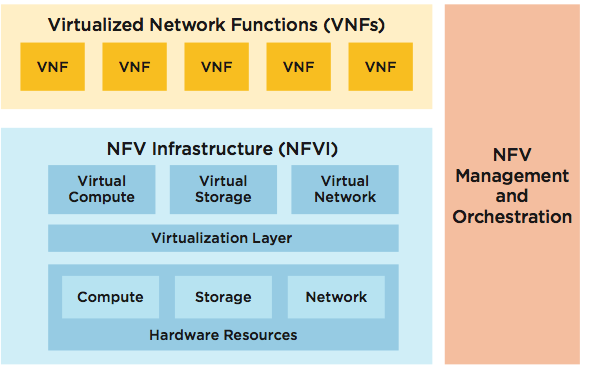
\includegraphics[scale=2]{etsi_arch}
 \caption{A schematic image representing the high level NFV architecture
   proposed by ESA.}
 \label{chap:prjan:img:etsi_arch}
\end{figure}

\begin{itemize}
 \item \textbf{Network Function Virtualization Infrastructure (NFVI)}: it's the
   heart of the whole computation component, and here three sub-domains can be
   identified: \todo{Expand this section}
\begin{itemize} 
 \item \textbf{Hypervisor domain} that is composed of the Virtual Compute, the
   Virtual Storage, and the Virtualization Layer. These components are used to
   virtualize the computational and storage resources, providing a layer for
   accessing it.
 \item \textbf{Compute domain} composed by the Physical Compute and the Physical
   Storage. These are the real resources which are virtualized via software.
 \item \textbf{Infrastructure domain} which has the Physical Network, and its
   virtualized counterpart as made available by the Virtualization Layer.
\end{itemize}

In conventional virtualization systems these resources are usually separated
from the host operating system, providing better isolation but wrost
performance. The ETSI infrastructure, instead, tries with container
virtualization technology to push for a better NFV responsiveness\todo{Check
  term - I don't think it actually exists}, removing the additional operating
system (called ``guest'' OS) required by the usual hypervisor-oriented approach.

To realize the required components, specific tools were suggested in the VNF
technical proposal: regarding the NFV (network infrastructure) domain
Docker-Compose was proposed as a viable solution, while to store PEP instances
docker swarm was described as a possible candidate.

We performed an accured analysis of the tools choosen based on their maturity,
on the community and on the technical support offered (e.g. user manuals,
developer documentation), which, at the end, commited us to choose different
tools from the suggested ones. A detailed description of the architectural
implementation can be found in chapter~\ref{chap:archimpl}.\todo{Include prof.
  survey about community components here}

\item \textbf{VNFs} this are the core components that perform packets
  manipulation. This components are design to be lightweight services able to
  elaborate a great amount of packets per seconds. Manupulation can be of two
  typologies: stateful or stateless. In the first case, a state is maintained,
  and the VNF can perform heuristics about data coming through it (especially
  useful to detect patterns in the data flow, e.g. DDos attacks). In the second
  case, no state is maintained, and every packet is treated without any
  particular assumption. Following the RFC 7665, the VNF are also called Service
  Function (SF)\footnote{From now on the two terminologies will be use in a
    interchangeable way.}. \todo{Add ref to chap about SFC?}

\item \textbf{NFV Management and Orchestration (MANO)} also known as NFV
  Orchestrator (NFVO) is responsible for the end-to-end management and
  orchestration of network services (NS), also called SFC. The MANO has
  different responsabilities, such as managing the
  istantiation/destruction/modification of the SFCs, that achieves interacting
  with the VIM.\todo{CITE: SDN/NFV-Based Mobile Packet Core Network
Architectures: A Survey}. Finally, the mano can integrate with 
Operational and Business Support Systems (OSS/BSS), \todo{Expand this part with 
the following papers: https://www.tandfonline.com/doi/abs/10.1057/jors.1995.176 
https://ieeexplore.ieee.org/abstract/document/6963800 
https://www.computer.org/csdl/proceedings/ifcsta/2009/3930/01/3930a466-abs.html}

\end{itemize}


\section{SFC}

\todo{Here it's missing an introduction about SFC and its terminology, need to 
include parts of RFC 7665}

\subsection{Packet transmission strategies}

When a packets are sent from a seder $S$, to a receiver $R$, they start
travelling to the backbone receiving appropriate in-hardware packet processing
before being received by $R$. During this elaboration, it is important to
maintain the transparency of the connection, so that the network users are not
aware of the packets elaboration at all. To perform that, many solutions are
available: TUN/TAP packet incapsulation, IP Encapsulation within IP or TCP
session recreation (know also as TCP split).

TUN/TAP and IP Encapsulation within IP (initially defined in RFC 2003 with the
aim to deliver IP packets over Mobile IP for mobile networks) maintain the
connection transparency incapsulating the packet in another one.
\begin{figure}[t]
  \centering 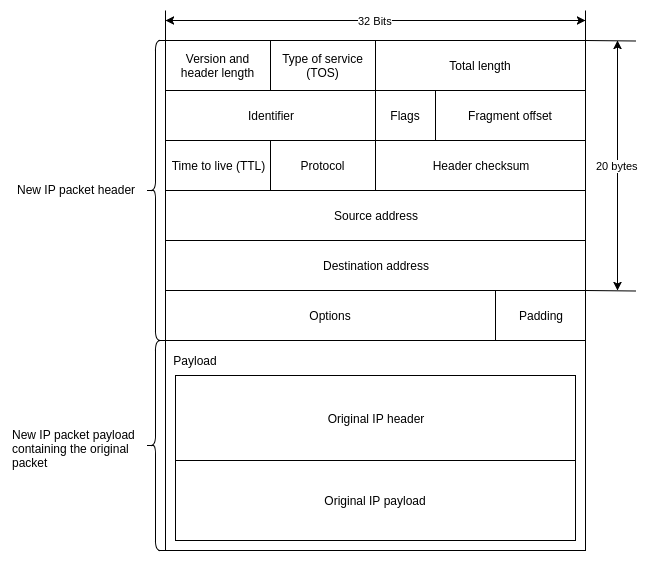
\includegraphics[scale=0.5]{IPoverIP}
  \caption[IP Encapsulation within IP packet schema]{A schema of IP
    Encapsulation within IP. Is noticeable how the original packet becomes the
    payload of a new one, thus being encapsulated. All the informations
    regarding the original packet remains untouched: when this kind of packet
    gets send from a machine to another, the OS will remove the new packet
    header and will present to the user-space program receiving the data its
    payload: a IP packet. Packets encapsulation can be applied with higher
    layers too, thus allowing for TCP and UDP packet incapsulation.}
  \label{chap:prjan:img:ip_over_ip}
\end{figure}


In this way, the original packet remains preserved and it becomes the new packet
payload, that can be elaborated and modified accordingly, until it gets
decapsulated and sent to $R$ eventually. When $R$ receives the packet, it is not
be aware of the packet elaboration, since all the original headers were
preserved (or slightly modified). In particular, IP Encapsulation within IP
allow the packets to make intermediate destinations that otherwise would not be
selected. TCP session recreation, instead, ``split'' the TCP session in two
endpoints: an Ingress, that manage the connection with the client and an Egress,
that communicate with the packet receiver creating a multi-overlay-hop path
where for each hop there is an possible indipendent TCP connection. In order to
achieve that, a session table needs to be established and continuously updated,
while TCP headers need to be accordingly modified to allow data transmission
through the Ingress and Egress points. Nonetheless, care should be given to
packets path: in order to avoid ill-calculated congestion windows, the incoming
packets need to follow the same (or an equivalent one) path for the same
instatiated connection. This phenomenom is based on the intermediate proxies
that create the route: it is the case, for example, when an intermediate node
sends back a spoofed ACK before the original packet is delivered to the real
consegnee. In this senario, the sender, unaware of the proxy, will miscalculate
the sending window based on the too low RTT. Other problems of TCP splitting are
reliability and security, especially because the end to end TCP logic is no
longer maintained: a server failure may cause to an unaware client to believe
that all the packets have reached the destination. TCP session recreation seems
burdersome and it doesn't seem to add any significant benefit at the first
sight, but it offers the flexibility to perform extensive packet manipulation:
since the packet its recreated every time at the Ingress and Egress points,
while in the Network Function Virtualization Infrastructure (NFVI), the original
packet can be stripped of its headers (that could be saved in the session table)
to slightly improve internal packet transmission. \todo{Insert TCP session
  recreation schema} On top of that, it offers the possibility to use different
TCP flavours, hence increasing the communication speed in heterogeneous networks
(e.g. in case of satellite connections TCP Hybla can be employed, while it is
known that HighSpeed TCP gives best results when applied in optical fiber-based
connections).

During the testbed development we first tried the TUN/TAP solution, that
revealed to be not completely transparent and with major performance drawbacks
(i.e. packet transmission in a LAN connection reached latencies of 50ms)
\todo{Explain the constraint of point-to-point connections, while we need
  dynamic SFC)}, so we choose to opt for a TCP session recreation solution,
implementing a little back-end with the aim of saving in a persistent storage
the SFC the packet has to perform and additional metadata.

\section{Available technologies in the market}

Before starting any effective work on the project it has been decided to 
perform an analysis of the possible technologies avvailable in the market, 
performing a choice between them and exploiting their possibile ``weak 
points''. Proceding with a top-down approach, the frameworks were choosen from 
the one that had the biggest role in the testbed to conclude with the 
less-important components.

\subsection{NFVI}

A critical component, as the MANO one, is the NFVI. Without it, network 
resources can't be allocated, and since our project was focused on dynamically 
allocating containerized applications on cloud platforms, we decided to start 
analizing the right framework for this component first.

\subsection{Openstack}
\label{chap:prjan:sec:openstack}
Created in ??\todo{Find out Openstack date of creation}, Openstack allows
on-permise cloud installations, using bare-metal resources to provide common
cloud services as object storage, virtual machine deploy, virtual networking.
Furthermore its modularity offers the possibility to add additional components,
even proprietary, to achieve a complete cloud solution.
\begin{figure}[t]
 \centering 
\includegraphics[scale=0.58]{openstack_logo}
 \caption{Openstack logo}
 \label{chap:prjan:img:openstack_logo}
\end{figure}



\todo{This section needs to be expanded a lot!!! In particular, we should put
  some focus about VNF and MANO, introducing them}





\subsubsection{Other technologies}\todo{Talk somehow of the other tecnhologies}
\paragraph{Openvswitch}
\paragraph{Openbaton} Patrocined by the Institute Fraunhofer, it's a 
open-source, customizable NFV MANO-compliant framework, that offers many
configurations options, and since it's written in Java, there is the possibility
to add components (plug-ins) dynamically. Openbaton can be installed as a normal
computer program (they offer packages for the most common distros) but it can be
deployed on Docker containers too. It's designed to work with cloud providers
like Amazon or Google Compute engine, but it offers compability with on-permise
cloud solutions like Openstack, where it deploys virtual machines using the API
the platform offers. It can store VNF configurations saved as TOSCA
YAML\todo{What does TOSCA mean? Find out} and it can handle multiple
PoPs\todo{Write down PoP meaning}. It offers a VNF lifecyle management
out-of-the-box, with the possibility to customize it based on the user needs.
Its modular design allows developers to change parts of the codebase with custom
ones, making the product really flexible to different platforms. Performing this
operation requires a deep knowlege of the framework though.
\begin{figure}[h]
 \centering 
\includegraphics[scale=0.45]{openbaton_logo}
 \caption{Openbaton logo}
 \label{chap:prjan:img:openbaton_logo}
\end{figure}

\paragraph{SDN?}

\chapter{Architectural implementation}
\label{chap:archimpl}
 

\appendix

%% FINE CONTENUTO TESI
%**************************************************************
% Materiale finale
%**************************************************************
\backmatter
\printglossaries

%**************************************************************
% Bibliografia
%**************************************************************

\cleardoublepage

\nocite{*}
\printbibliography

\bibbycategory % equivale a dare un \printbibliography per ogni categoria




\end{document}
